\documentclass{beamer}
\usetheme{Madrid}

\usepackage[utf8]{inputenc} % указывает кодировку документа
\usepackage[T2A]{fontenc} % указывает внутреннюю кодировку TeX 
\usepackage[main=russian,english]{babel} % указывает язык документа
\usepackage{booktabs}
\usepackage{graphicx}
\usepackage{hyperref}
\hypersetup{
     colorlinks   = true,
     citecolor    = blue
}
\usepackage[ruled,vlined]{algorithm2e}
\usepackage{booktabs}
\usepackage{multicol}
\usepackage{lipsum}
\usepackage{mwe}

\title[Методы оптимизации]{Стохастические квазиньютоновские методы оптимизации в контексте глубоких нейронных сетей}
\author[]{А. Жогов \and М. Сысак \and Б. Усеинов}
\institute[МФТИ]{Московский физико-технический институт, Москва, Россия}

\centering
\date{26 мая 2020 г.}
\begin{document}
\setbeamertemplate{caption}{\raggedright\insertcaption\par}
\setbeamerfont{caption}{size=\small}
\setlength{\abovecaptionskip}{-2pt}
\setlength{\belowcaptionskip}{6pt}
\maketitle

%--------------------------------------------------------------------------

\begin{frame}{Постановка задачи}
\begin{itemize}
    \item Нейронные сети являются передовыми методами во множестве задач машинного обучения.
    \item Квазиньютоновские методы широко используются в выпуклой оптимизации.
    \item В глубинном обучении стохастические модификации квазиньютоновских методов используются редко из-за их неустойчивости.
\end{itemize}
\end{frame}

%--------------------------------------------------------------------------

\begin{frame}{Постановка задачи}
\begin{itemize}
    \item $\mathcal{X} = \{\mathbf{x}_i, y_i\}_1^n$~--- выборка, $f(\mathbf{x}_i, \theta)$~--- нейронная сеть, функция потерь:
    $$\mathcal{L}(\mathbf{p}, y) = -\log p_y$$
    \item Задача оптимизации:
    $$\min_\theta F_\mathcal{X}(\theta) \triangleq \frac1n \sum_{i=1}^n \mathcal{L}(f(x_i, \theta), y_i)$$
    \item Минибатч $\mathcal{X}' \subset \mathcal{X},\, s = |\mathcal{X}'| \ll |\mathcal{X}|$
    \item Вспомогательная задача
    $$\min_\theta F_{\mathcal{X}'}(\theta) \triangleq \frac1s \sum_{j=1}^s \mathcal{L}(f(x_{i_j}, \theta), y_{i_j})$$
\end{itemize}
\end{frame}

%--------------------------------------------------------------------------

\begin{frame}{Методы}
\framesubtitle{SGD | SGD-Momentum}
\begin{itemize}
    \item На каждой итерации генерируется минибатч $\mathcal{X}_t' \subset \mathcal{X}$
    \item Шаг стохастического градиентного спуска (SGD):
    $$\theta_{k+1} = \theta_k - \eta \nabla F_{\mathcal{X}_t'} (\theta_k)$$
    \item Шаг SGD-Momentum:
    $$\theta_{k+1} = \theta_k - \eta \nabla F_{\mathcal{X}_t'}(\theta_k) + \beta (\theta_k - \theta_{k+1})$$
\end{itemize}
\end{frame}

%--------------------------------------------------------------------------

\begin{frame}{Методы}
\framesubtitle{Adam}
\begin{itemize}
    \item На каждой итерации генерируется минибатч $\mathcal{X}_t' \subset \mathcal{X}$
    \item Вычисляется градиент $g_{t+1} = \nabla F_{\mathcal{X}_t'}(\theta_t)$ и обновляются скользящие средние
    $$m_{t+1} = \beta_1  m_t + (1 - \beta_1) g_{t+1} \quad v_{t+1} = \beta_2  v_t + (1 - \beta_2) g_{t+1}^2$$
    \item Поправка на смещение
    $$\hat{m}_{t+1} = m_{t+1} / (1 - \beta_1^{t+1}) \quad \hat{v}_{t+1} = v_{t+1} / (1 - \beta_2^{t+1})$$
    \item Обновление целевой переменной
    $$\theta_{t+1} = \theta_t - \eta \cdot \hat{m}_{t+1}/(\sqrt{\hat{v}_{t+1}} + \varepsilon)$$
\end{itemize}
\end{frame}

%--------------------------------------------------------------------------

\begin{frame}{Методы}
\framesubtitle{Multi-Batch LBFGS}
\begin{itemize}
    \item На каждой итерации генерируется минибатч $\mathcal{X}'_k \subset \mathcal{X}$
    \item Требование пересечения минибатчей: 
    $$O_k = \mathcal{X}_{k+1}' \cap \mathcal{X}_k' \quad  |O_k| = l < s = |\mathcal{X}_k'|$$
    \item Квазиньютоновское уравнение:
    $$y_{k+1} = \nabla F_{O_k}(\theta_{k+1}) - \nabla F_{O_k}(\theta_k) \quad s_{k+1} = \theta_{k+1} - \theta_k$$
    $$s_{k+1} = H_{k+1}y_{k+1}$$
    \item Вычисление оценки гессиана $H_{k+1}$ с помощью процедуры two\_loop\_recursion
    \item Обновление целевой переменной
    $$\theta_{k+1} = \theta_k - \eta H_k \nabla F_{\mathcal{X}_k'}(\theta_k)$$
\end{itemize}
\end{frame}

%--------------------------------------------------------------------------

\begin{frame}{Методы}
\framesubtitle{SGD-BB}
\begin{itemize}
    \item Эпоха~--- $\left\lceil\dfrac{|\mathcal{X}|}{|\mathcal{X}'|}\right\rceil \triangleq T$ итераций 
    \item $k$~--- номер эпохи, $t$~--- номер итерации, минибатч $\mathcal{X}_{k, t}'$
    \item Обновление переменной и оценки градиента:
    $$\theta_{k, 0} = \theta_{k-1, T} \quad \theta_{k, t+1} = \theta_{k, t} - {\eta}_k \nabla F_{\mathcal{X}_{k, t}'}(\theta_{k, t})$$
    $$g_{k, t+1} = (1 - \beta) g_{k, t} + \beta \nabla F_{\mathcal{X}_{k, t}'}(\theta_{k, t})$$
    \item Обновление размера шага:
    $$y_k = g_{k, T} - g_{k-1, T} \quad s_k = T^{-1}(\theta_{k, T} - \theta_{k-1, T})$$
    $$\eta_{k+1} = \frac{\|s_k\|_2^2}{|s_k^Ty_k|}$$
\end{itemize}
\end{frame}

%--------------------------------------------------------------------------

\begin{frame}{Результаты}
\framesubtitle{Эксперимент с MNIST}


\begin{table}[h!]
\caption{Архитектура нейронной сети в эксперименте с MNIST}
\centering
\begin{tabular}{{l|l}}
\toprule
№ & Слой \\
\midrule
0:~вход & $28\times28$ изображение, $1\times784$ \\
1: & Полносвязный, $(784, 128)$, ReLU \\
2: & Полносвязный, $(128, 64)$, ReLU \\
3:~выход & Полносвязный, $(64, 10)$, LogSoftmax \\
\bottomrule
\end{tabular}
\label{MNISTnet}
\end{table}

\end{frame}

%--------------------------------------------------------------------------

\begin{frame}{Результаты}
\framesubtitle{Эксперимент с MNIST}
\begin{table}[h!]
\caption{Время, затраченное на 15 эпох обучения}
\centering
\begin{tabular}{c|c|c|c|c}
\toprule
\textbf{Метод} & SGD & SGD-Momentum & Adam & SGD-BB \\ 
\midrule
\textbf{Время, мин} & \textbf{2.81} & 3.10 & 3.80 & 3.33 \\
\bottomrule
\end{tabular}
\end{table}

\begin{figure}
    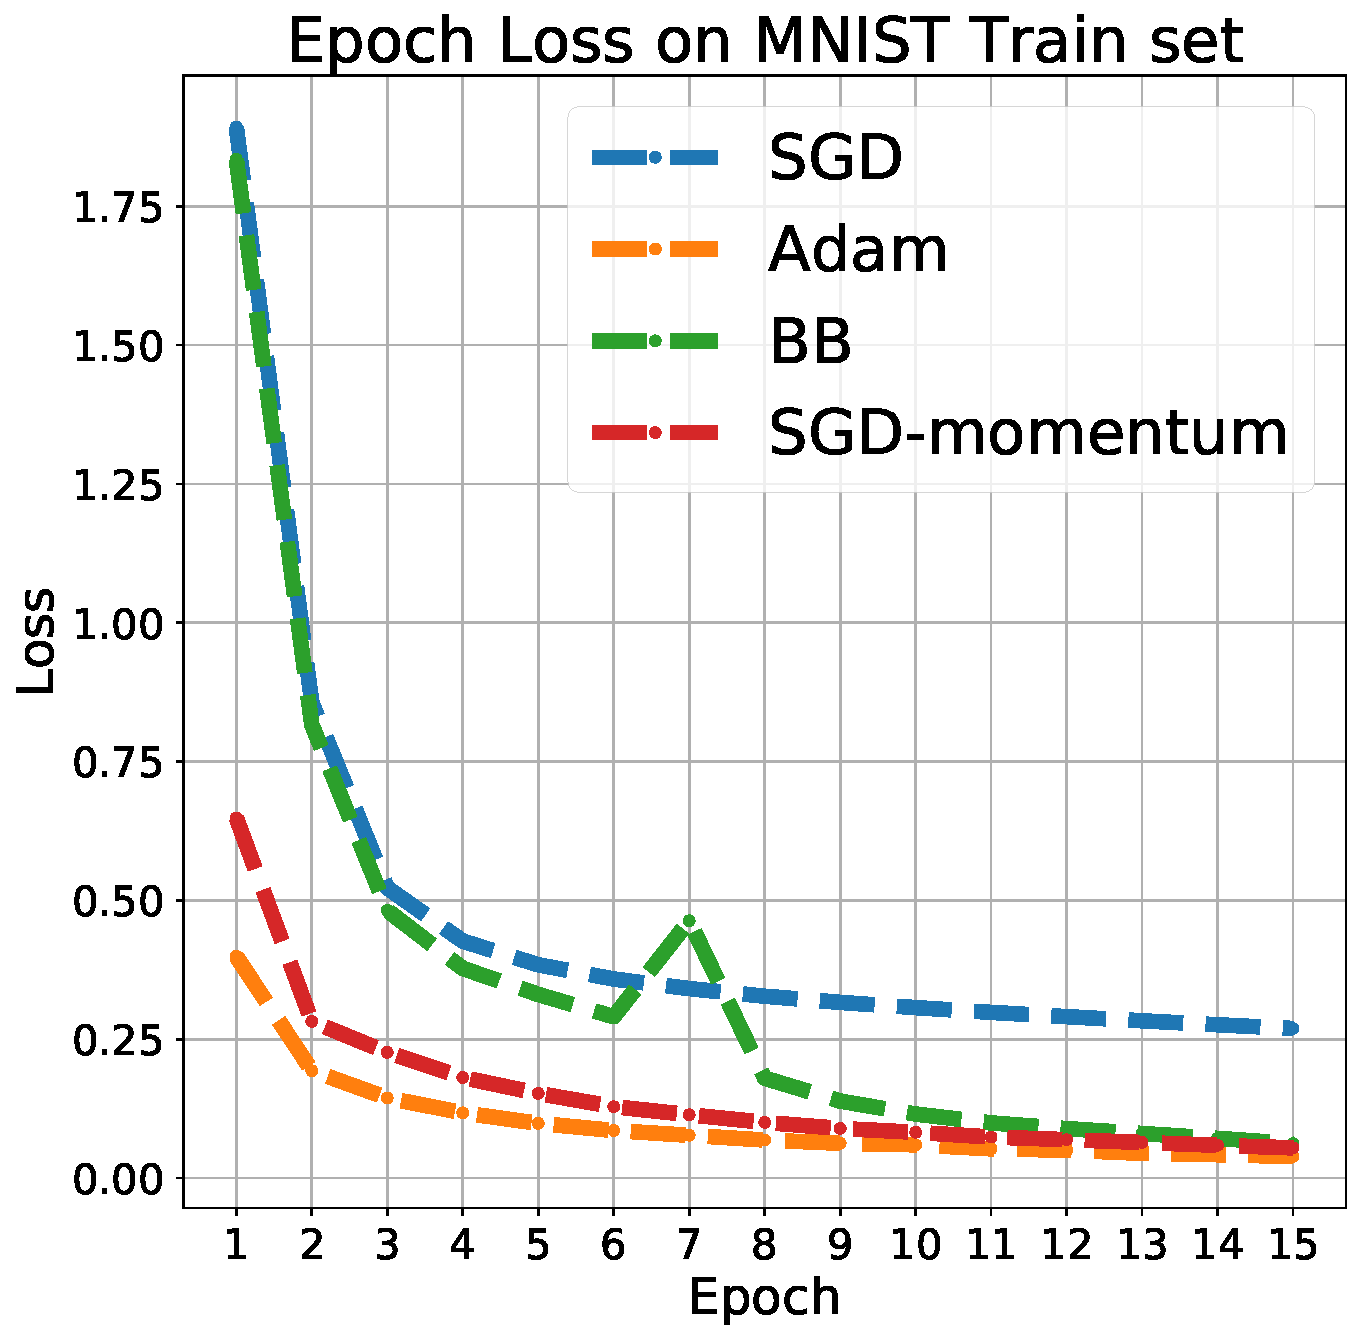
\includegraphics[height=.3\textwidth]{mnist_train_losses.pdf}
    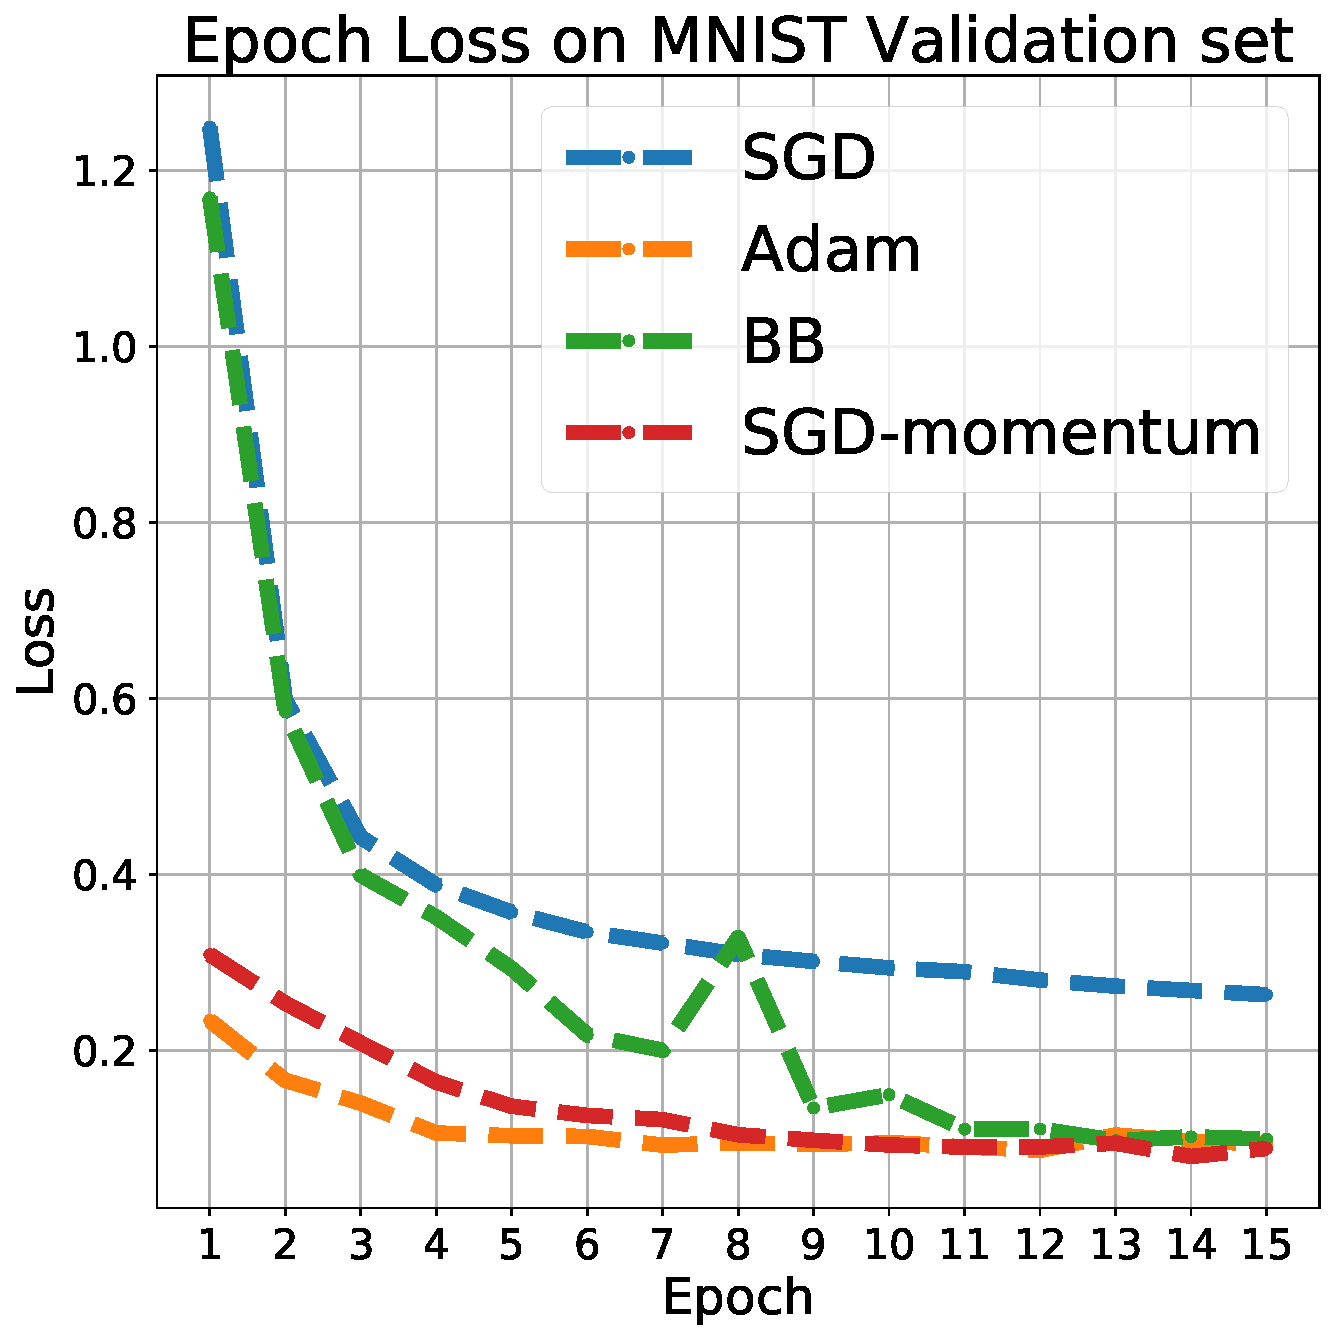
\includegraphics[height=.3\textwidth]{mnist_val_losses.pdf}
    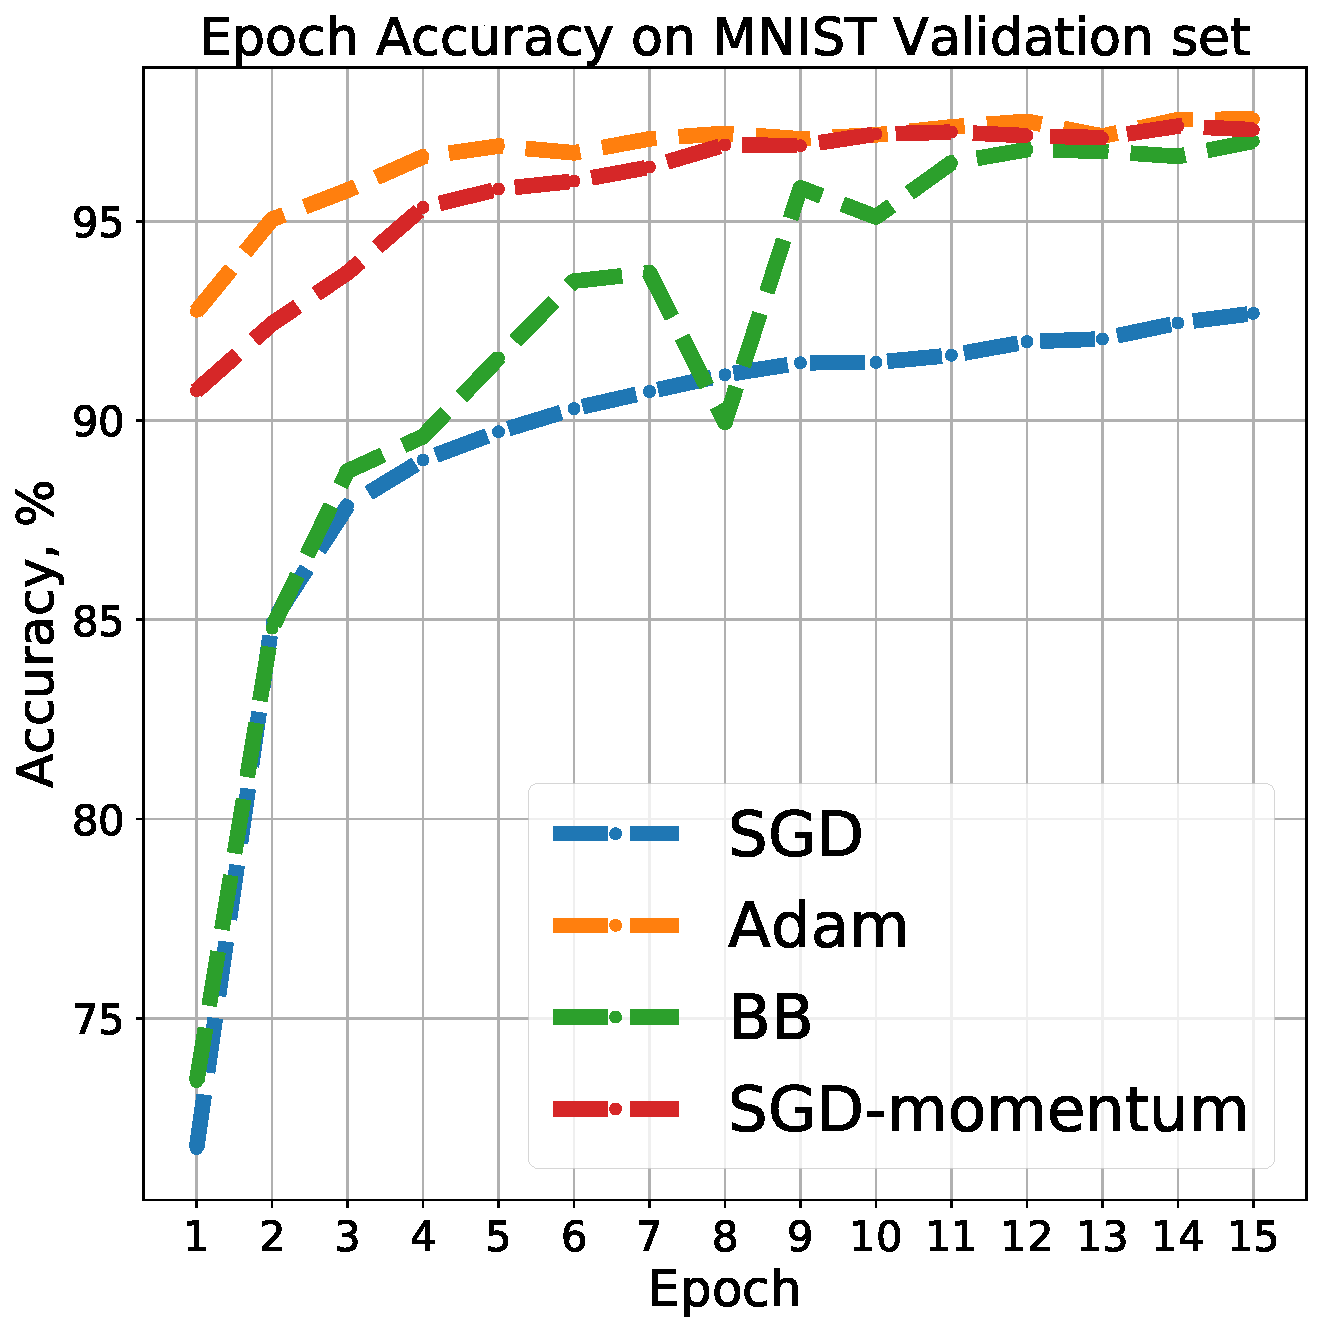
\includegraphics[height=.3\textwidth]{mnist_val_accuracy.pdf}
\caption{Графики сходимости методов}
\end{figure}
\end{frame}

%--------------------------------------------------------------------------

\begin{frame}{Результаты}
\framesubtitle{Эксперимент с CIFAR-10}
\begin{table}[h!]
\caption{Архитектура нейронной сети в эксперименте с CIFAR-10}
\centering
\begin{tabular}{{l|l}}
\toprule
№ & Слой \\
\midrule
0:~вход & \text{$32\times32$ изображение} \\
1: & Сверточный, $(6,\ 5\times5,\ 1)$, ReLU \\
2: & Субдискретизирующий (макс.), $(2\times2, 1)$\\
3: & Сверточный, $(16,\ 5\times5,\ 1)$, ReLU \\
4: & Полносвязный, $(4096, 1000)$, ReLU \\
5:~выход & Полносвязный, $(1000,10)$, LogSoftmax\\
\bottomrule
\end{tabular}
\label{CIFAR10net}
\end{table}
\end{frame}

%--------------------------------------------------------------------------

\begin{frame}{Результаты}
\framesubtitle{Эксперимент с CIFAR-10}
\begin{table}
\caption{Время, затраченное на 15 эпох обучения}
\centering
\begin{tabular}{c|c|c|c|c|c}
\toprule
\textbf{Метод} & MB-LBFGS & Adam & SGD & SGD-Momentum & SGD-BB \\ 
\midrule
\textbf{Время, мин} & 6.37 & 5.35 & 5.19 & 5.40 & \textbf{5.16} \\
\bottomrule
\end{tabular}
\end{table}
\begin{figure}
    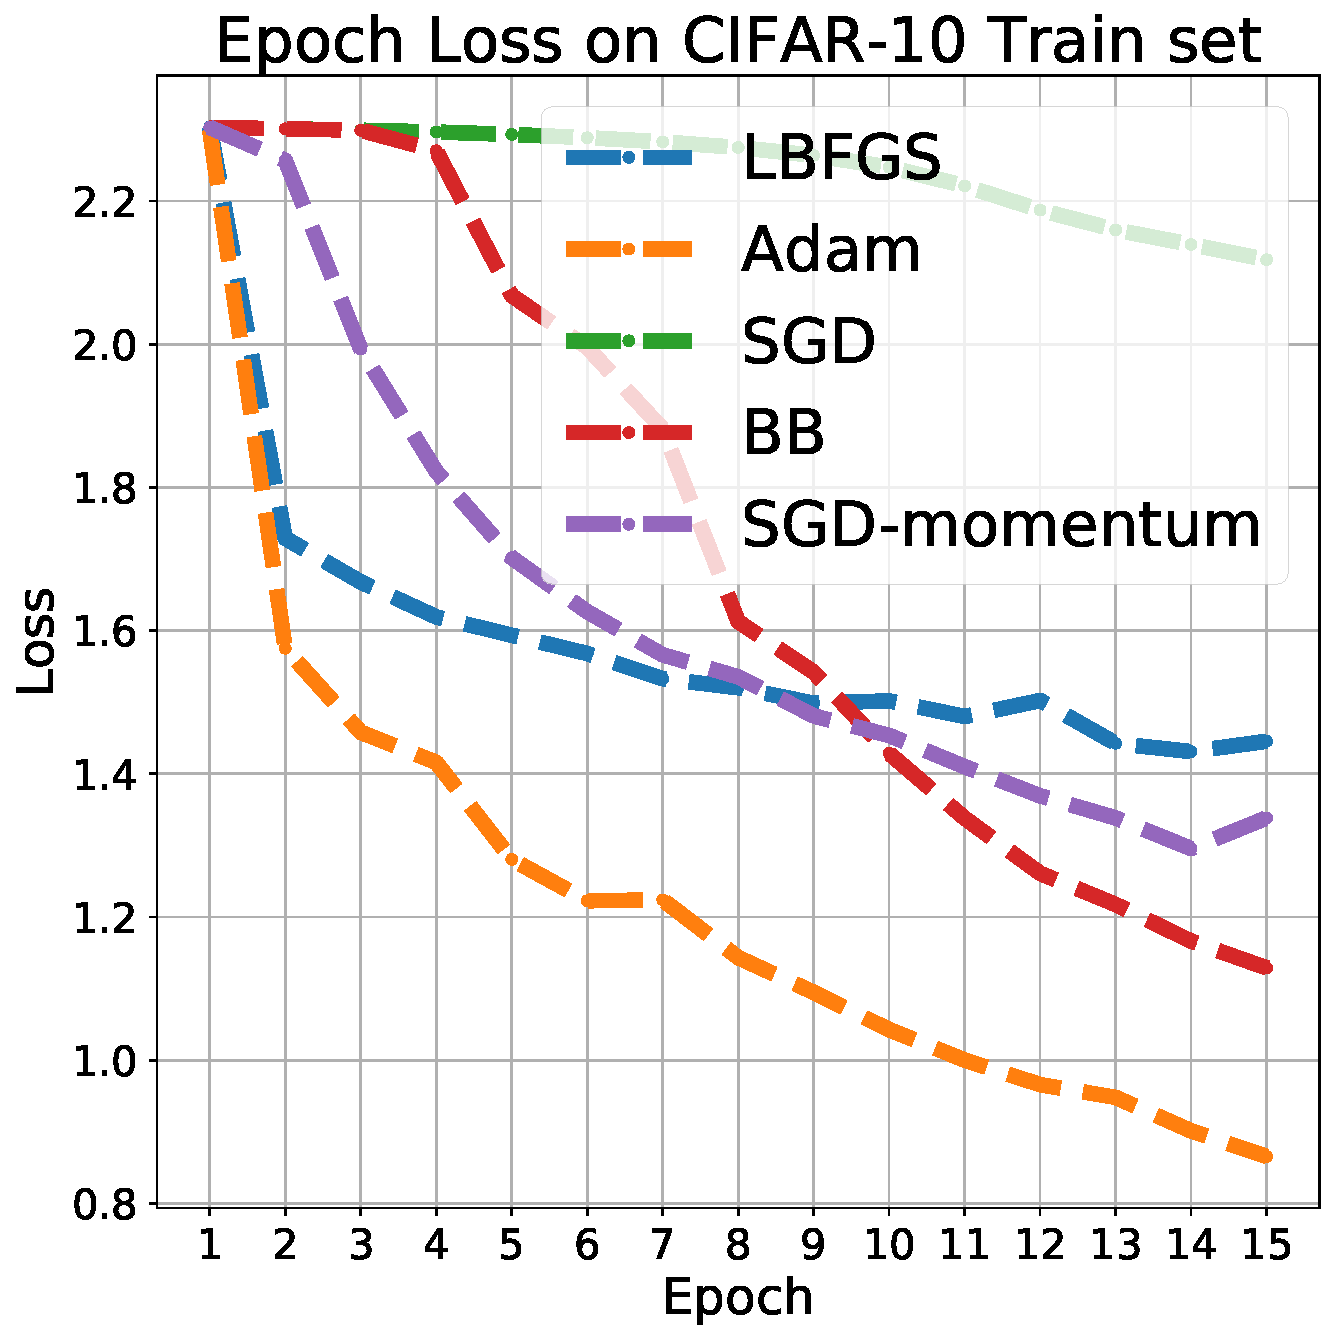
\includegraphics[height=.3\textwidth]{cifar_train_losses.pdf}
    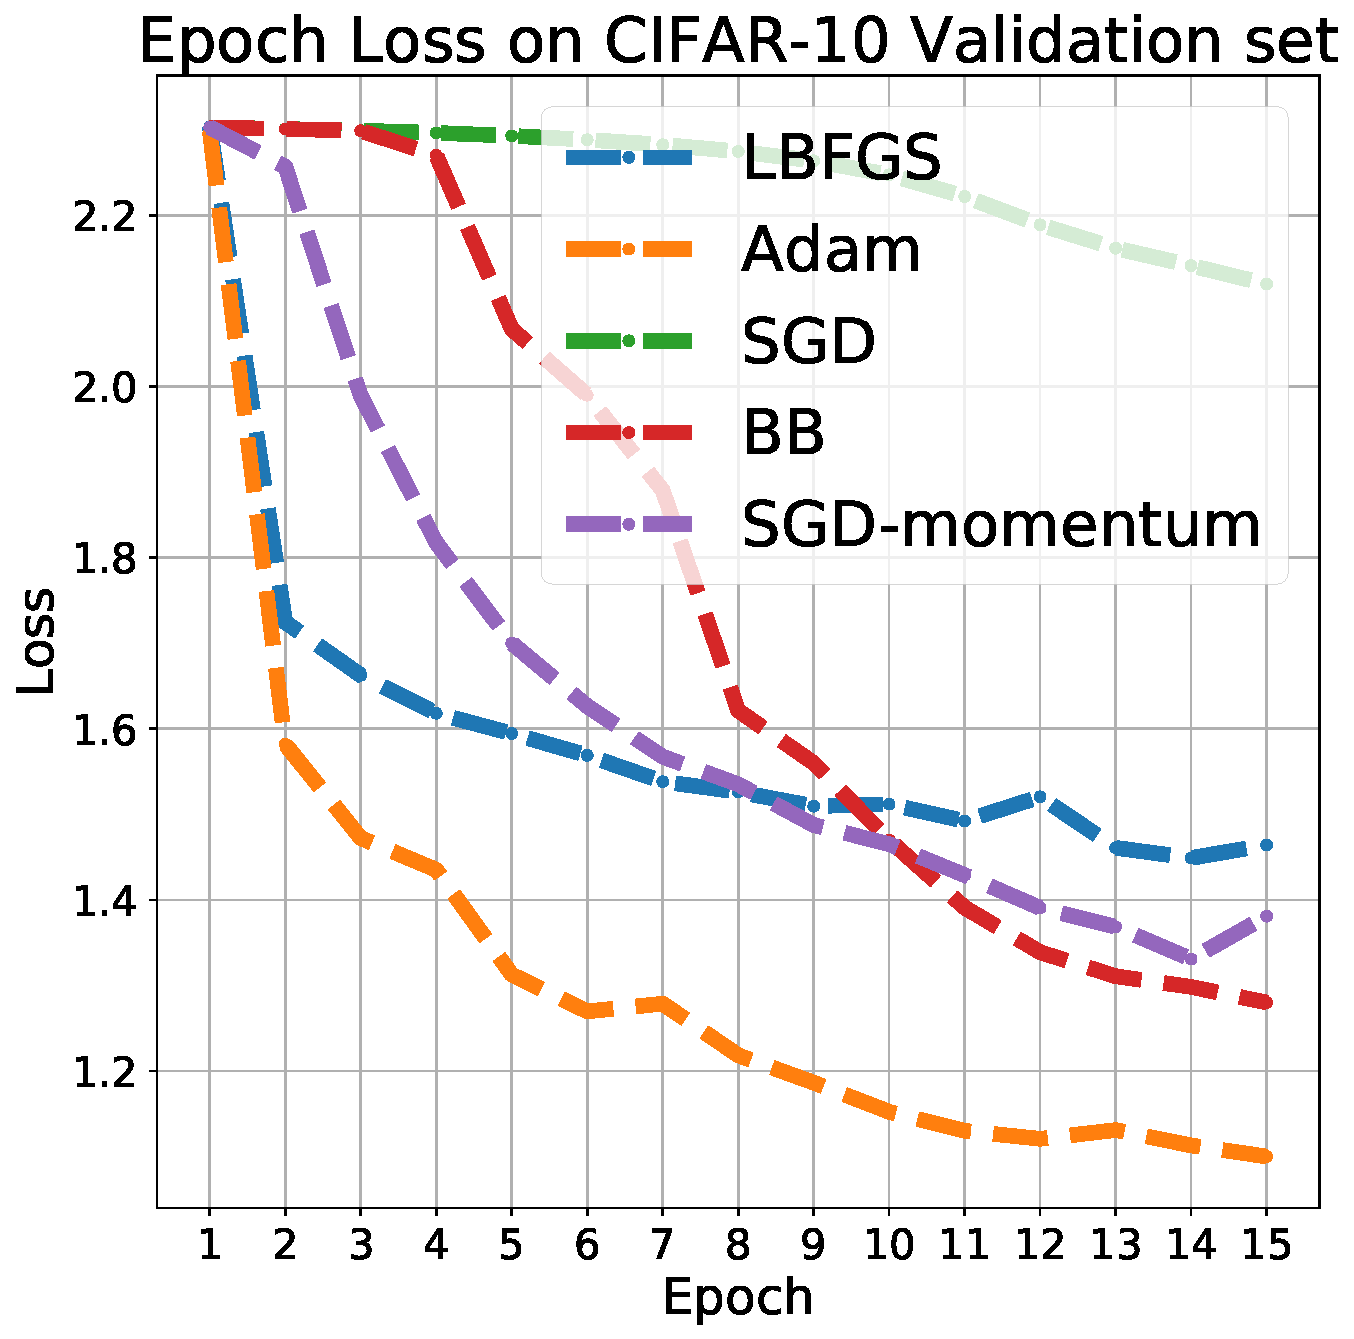
\includegraphics[height=.3\textwidth]{cifar_val_losses.pdf}
    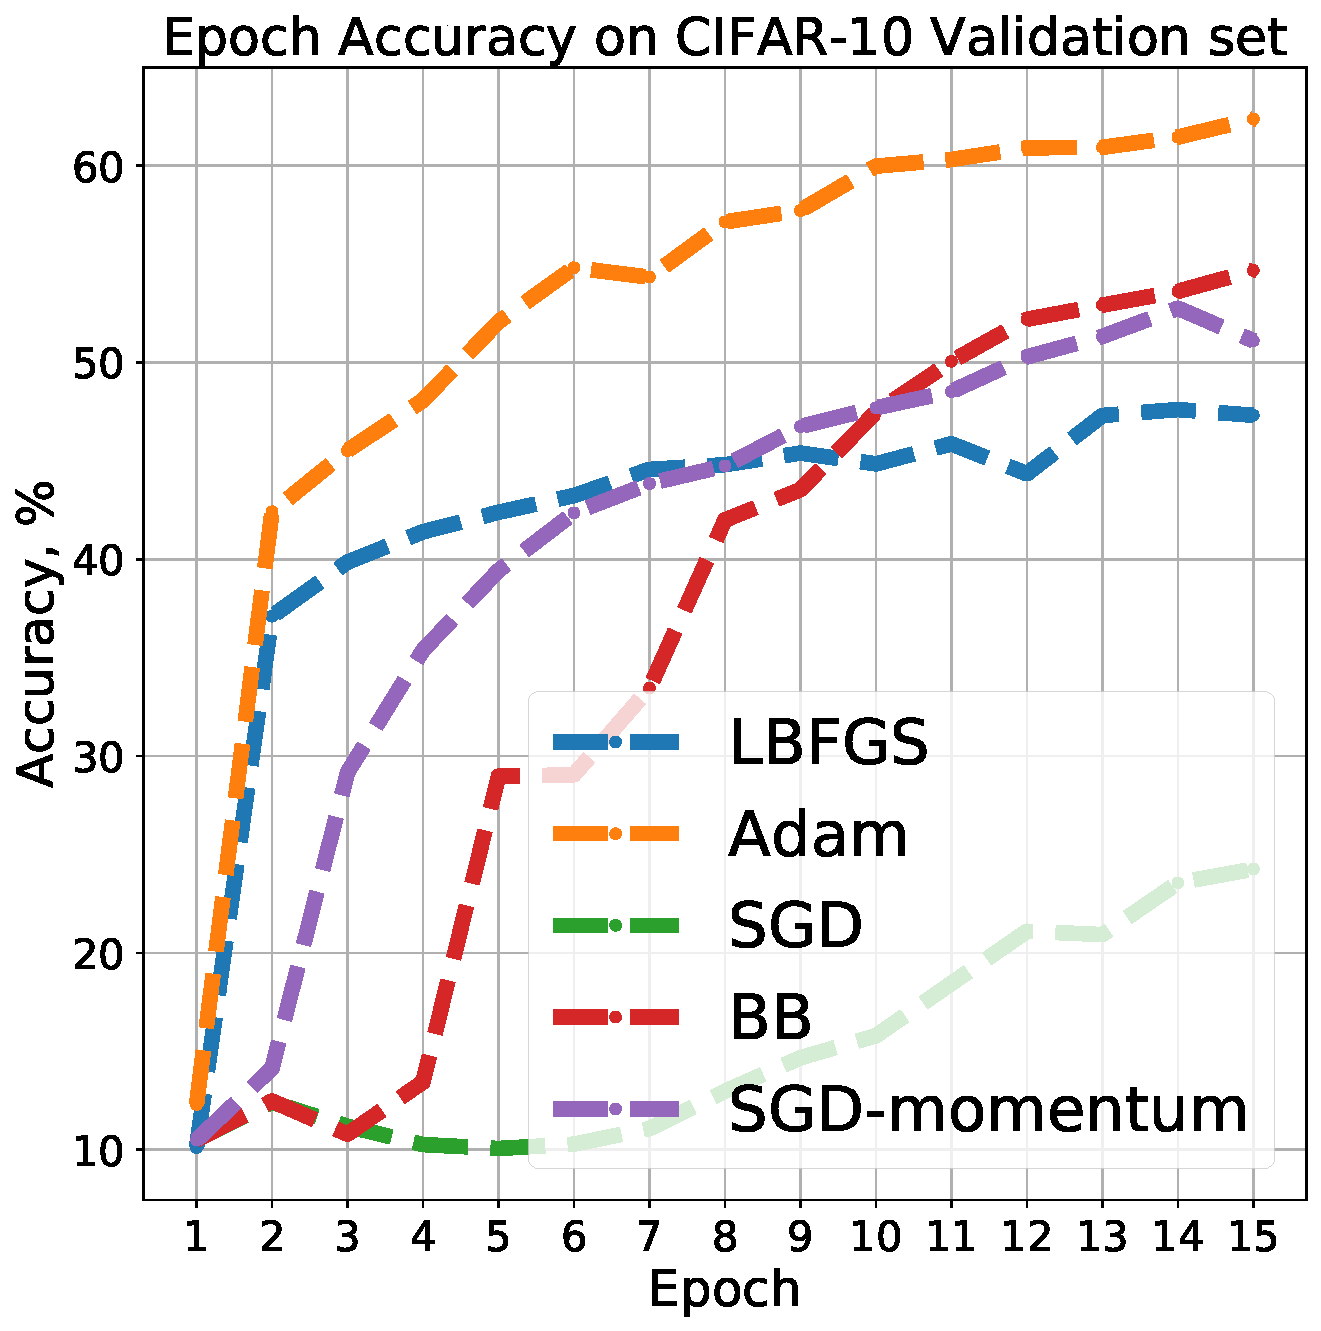
\includegraphics[height=.3\textwidth]{cifar_val_accuracy.pdf}
\caption{Графики сходимости методов}
\end{figure}
\end{frame}


%--------------------------------------------------------------------------

\begin{frame}{Выводы}
\begin{itemize}
    \item Квазиньютоновские методы сопоставимы с Adam и SGD-Momentum по качеству решения.
    \item SGD требует больше итераций для сходимости.
\end{itemize}
\vspace{10pt}
\begin{itemize}
    \item Все методы кроме MB-LBFGS затрачивают сопоставимое количество времени.
    \item MB-LBFGS работает на $20\%$ дольше.
\end{itemize}

\end{frame}

%--------------------------------------------------------------------------

\end{document}
